\documentclass[11pt,a4paper]{article}

\usepackage[margin=2.0cm]{geometry}
\usepackage[T1]{fontenc}
\usepackage[utf8]{inputenc}
\usepackage{lmodern}
\usepackage{microtype}
\usepackage{amsmath,amssymb,mathtools,bm}
\usepackage{booktabs,tabularx,longtable,array,multirow}
\usepackage{graphicx}
\usepackage{caption,subcaption}
\usepackage{enumitem}
\usepackage{xcolor}
\usepackage{hyperref}
\usepackage{cleveref}
\usepackage[backend=biber,style=numeric-comp,sorting=none]{biblatex}
\addbibresource{references.bib}
\usepackage{fancyhdr}
\usepackage{titlesec}
\usepackage{float}
\usepackage{siunitx}
\usepackage{url}
\usepackage[most]{tcolorbox}
\usepackage{tikz}
\usetikzlibrary{arrows.meta,positioning,fit,calc,shapes.geometric,backgrounds}
\usepackage{listings}

\definecolor{deepblue}{RGB}{28,63,105}
\definecolor{deepgreen}{RGB}{38,105,79}
\definecolor{deeporange}{RGB}{170,92,20}
\definecolor{deepred}{RGB}{145,52,52}
\definecolor{softblue}{RGB}{232,241,250}
\definecolor{softgreen}{RGB}{235,247,240}
\definecolor{softorange}{RGB}{253,243,226}
\definecolor{softred}{RGB}{252,235,235}
\definecolor{softgray}{RGB}{245,246,248}

\hypersetup{
  colorlinks=true,
  linkcolor=deepblue,
  citecolor=deepgreen,
  urlcolor=deeporange,
  pdftitle={Geometry-MMALS G1: Replicated Context Geometry and the Specification of Functional Routing},
  pdfauthor={Guillaume Harbonnier}
}

\pagestyle{fancy}
\fancyhf{}
\lhead{Geometry-MMALS G1}
\rhead{v1.0.9 results and v1.1.0 specification}
\cfoot{\thepage}
\setlength{\headheight}{14pt}

\titleformat{\section}{\Large\bfseries\color{deepblue}}{\thesection}{0.8em}{}
\titleformat{\subsection}{\large\bfseries\color{deepgreen}}{\thesubsection}{0.8em}{}
\titleformat{\subsubsection}{\normalsize\bfseries\color{deeporange}}{\thesubsubsection}{0.8em}{}

\setlist[itemize]{leftmargin=1.5em,itemsep=2pt,topsep=3pt}
\setlist[enumerate]{leftmargin=1.7em,itemsep=3pt,topsep=3pt}
\renewcommand{\arraystretch}{1.14}
\newcolumntype{Y}{>{\raggedright\arraybackslash}X}
\newcolumntype{C}{>{\centering\arraybackslash}X}
\newcommand{\MMALS}{\textsc{MMALS}}
\newcommand{\R}{\mathbb{R}}
\newcommand{\E}{\mathbb{E}}
\newcommand{\loss}{\mathcal{L}}
\newcommand{\norm}[1]{\left\lVert #1 \right\rVert}
\newcommand{\softmax}{\operatorname{softmax}}
\newcommand{\relu}{\operatorname{ReLU}}
\newcommand{\KL}{\operatorname{KL}}

\newtcolorbox{plainbox}[1][]{
  title={#1},colback=softblue,colframe=deepblue!45,boxrule=0.6pt,arc=2pt,
  left=8pt,right=8pt,top=7pt,bottom=7pt
}
\newtcolorbox{positivebox}[1][]{
  title={#1},colback=softgreen,colframe=deepgreen!45,boxrule=0.6pt,arc=2pt,
  left=8pt,right=8pt,top=7pt,bottom=7pt
}
\newtcolorbox{warningbox}[1][]{
  title={#1},colback=softorange,colframe=deeporange!50,boxrule=0.6pt,arc=2pt,
  left=8pt,right=8pt,top=7pt,bottom=7pt
}
\newtcolorbox{criticalbox}[1][]{
  title={#1},colback=softred,colframe=deepred!50,boxrule=0.6pt,arc=2pt,
  left=8pt,right=8pt,top=7pt,bottom=7pt
}
\newtcolorbox{mathbox}[1][]{
  title={#1},colback=softgray,colframe=black!30,boxrule=0.5pt,arc=1pt,
  left=8pt,right=8pt,top=7pt,bottom=7pt
}

\begin{document}

\begin{titlepage}
\centering
\vspace*{0.7cm}
{\Huge\bfseries\color{deepblue} Geometry-MMALS G1\par}
\vspace{0.25cm}
{\LARGE Replicated Context Geometry\par}
\vspace{0.15cm}
{\LARGE and the Specification of Functional Routing\par}
\vspace{0.35cm}
{\Large Results of v1.0.9 and complete research specification for v1.1.0\par}
\vspace{0.5cm}
{\large Technical article and repository update\par}
\vspace{0.9cm}
{\Large Guillaume Harbonnier\par}
\vspace{0.2cm}
{\normalsize Independent MMALS research program\par}
\vspace{0.15cm}
{\normalsize \href{https://github.com/gharbonnier78/geometry-mmalls-g1}{github.com/gharbonnier78/geometry-mmalls-g1}\par}
\vspace{0.6cm}
{\normalsize Evidence snapshot: five matched-compute model seeds, RotatedMNIST, June 2026\par}
\vfill
\begin{minipage}{0.93\textwidth}
\small
\textbf{Epistemic status.} Geometry-MMALS G1 v1.0.9 provides the first replicated candidate evidence that the system can learn an ordered and held-out-decodable latent context representation. Across five seeds, the aligned four-dimensional context objective improves trained-angle context distance-order correlation by $0.107$ with a 95\% seed interval of $[0.029,0.185]$, reduces context stress by $0.042$, improves held-out-source factor decoding by $0.132$ in $R^2$, and reduces angle error by about $5^\circ$. The effect does not reliably propagate to route geometry, host synthesis, classification accuracy, forgetting, or causal specificity. The paper therefore separates three levels of evidence: representational geometry, functional mediation, and operational value. Only the first is reached at candidate level. The proposed v1.1.0 experiment is designed to build and falsify the missing bridge from context geometry to routing and differentiated host activity. No claim of final C1--C6 qualification, domain-general geometry, quantum computation, or quantum advantage is made.
\end{minipage}
\vfill
\end{titlepage}

\begin{abstract}
Geometry-MMALS G1 studies whether a modular continual-learning system can acquire an internal geometry that reflects a known factor of variation, generalizes to unseen source identities, causally controls routing, and eventually improves learning or retention. The system contains a frozen sensory representation $z_0$, an inferred context $c$, a route $r$ over functional hosts, a routed synthesis $z_M$, and a classifier. Version 1.0.9 evaluates three matched methods across five model seeds: a no-geometry control, a globally aligned model with a legacy route target, and a globally aligned model with a stationary route target.

The replicated positive result is narrow but significant. Relative to the no-geometry control, the stationary full-alignment treatment increases trained-angle context distance-order correlation by $0.107$ with 95\% seed interval $[0.029,0.185]$ and reduces context stress by $0.042$ with interval $[-0.084,-0.001]$. All five seeds exhibit a positive context-order effect. On source identities excluded from fitting, the inferred context improves angle decoding by $0.132$ in $R^2$ and approximately $5^\circ$ in mean absolute error. In contrast, route-order effects do not replicate, synthesis geometry is unchanged, predictive accuracy and forgetting remain neutral, causal specificity is below the preregistered threshold, and the stationary route target does not outperform the legacy target.

The central conclusion is therefore that Geometry-MMALS can construct a grounded representational context geometry, but the current router does not demonstrably convert that geometry into functional or operational control. This paper explains that result at two levels: an intuitive account accessible to non-specialists and a complete mathematical account. It then specifies v1.1.0 as a controlled comparison among an MLP router, a low-capacity linear router, and a prototype-energy router, using both nominal simplex geometry and a new functional optimal-transport metric over hosts. The specification includes causal interventions, host-ecology measurements, matched-compute controls, statistical gates, falsification conditions, and the longer G1$\rightarrow$G2$\rightarrow$G3 roadmap.
\end{abstract}

\tableofcontents
\clearpage

\section{What the program builds, in concrete terms}

\begin{plainbox}[A simple picture before the mathematics]
Imagine training a system to recognize handwritten digits rotated to $-60^\circ$, $-30^\circ$, $0^\circ$, $30^\circ$, and $60^\circ$. The system sees one rotation regime after another, as a continual learner rather than as a model trained once on a fully mixed dataset.

Inside the system, several components cooperate:
\begin{itemize}
\item $z_0$ is the \emph{sensory view}: a frozen representation of the image. It does not change during the Geometry-MMALS experiment.
\item $c$ is the \emph{inferred context}: a small vector of four numbers intended to summarize ``what situation am I in?''
\item $r$ is the \emph{route}: a probability distribution describing how much each specialist, or host, should contribute.
\item the hosts are small functional subnetworks that transform the sensory representation in different ways;
\item $z_M$ is the weighted synthesis of their outputs, and the classifier produces the final digit prediction.
\end{itemize}
\end{plainbox}

\subsection{The central question, stated simply}

The first question is whether the inferred context learns to represent rotation in a geometrically coherent way. If the same digit is seen at $0^\circ$ and $30^\circ$, the corresponding contexts should normally be closer to each other than either is to the context at $-60^\circ$. A previously unseen intermediate angle such as $-15^\circ$ should occupy a position between $-30^\circ$ and $0^\circ$ rather than an arbitrary location.

This is called \emph{representational geometry}: relations in the internal space reflect relations in the external world. It is not enough to draw a visually attractive projection. The order must survive held-out source identities, statistical controls, and repeated model initializations.

\subsection{What v1.0.9 demonstrated}

\begin{positivebox}[The good news]
Across five independent model initializations, the aligned training objective produces a more ordered four-dimensional context space. The effect is reproducible rather than a lucky seed. More importantly, when the model is evaluated on source images not used to fit the geometric decoder, the context predicts the rotation angle with about $5^\circ$ less error. The context has therefore learned a relation that transfers across image identities.
\end{positivebox}

\begin{warningbox}[The unresolved problem]
The ordered context does not reliably produce an ordered route. Classification accuracy, forgetting, and synthesis geometry do not improve. The system has built a useful map, but the downstream decision process does not yet demonstrate that it uses the map in an operationally meaningful way.
\end{warningbox}

A useful analogy is an employee who receives a precise geographic map but continues to distribute files using other habits. The map is accurate and generalizes to new locations, yet it does not visibly determine the employee's decisions. Scientifically, the analogy has one caveat: the employee may truly ignore the map, or our current way of measuring the employee's decisions may fail to recognize functionally equivalent choices. Version 1.1.0 is designed to distinguish these possibilities.

\subsection{Three levels of evidence}

\begin{center}
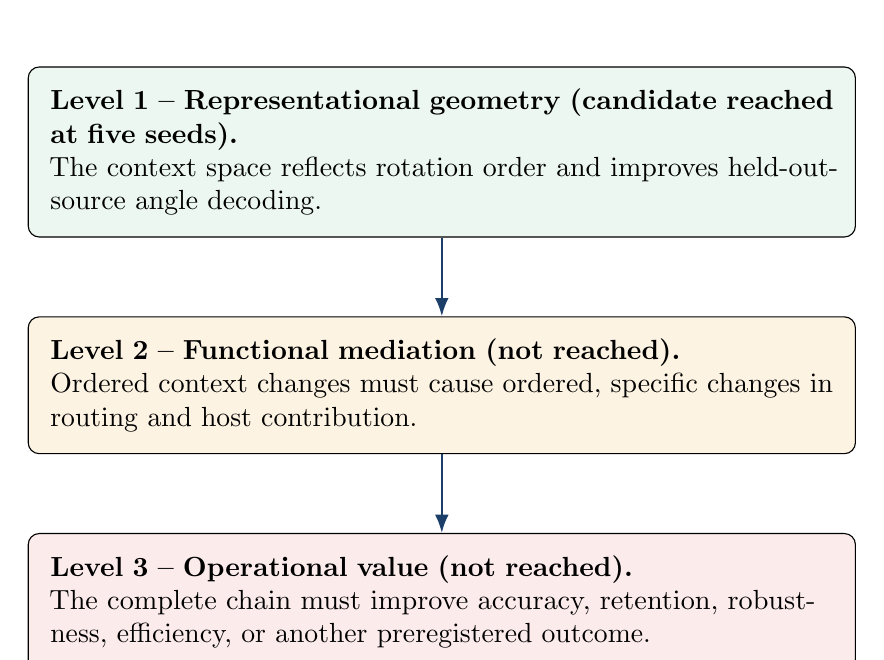
\begin{tikzpicture}[
node distance=1.0cm,
box/.style={draw,rounded corners,text width=0.82\textwidth,minimum height=1.2cm,align=left,inner sep=8pt},
arr/.style={-Latex,thick,deepblue}
]
\node[box,fill=softgreen] (l1) {\textbf{Level 1 -- Representational geometry (candidate reached at five seeds).}\\The context space reflects rotation order and improves held-out-source angle decoding.};
\node[box,fill=softorange,below=of l1] (l2) {\textbf{Level 2 -- Functional mediation (not reached).}\\Ordered context changes must cause ordered, specific changes in routing and host contribution.};
\node[box,fill=softred,below=of l2] (l3) {\textbf{Level 3 -- Operational value (not reached).}\\The complete chain must improve accuracy, retention, robustness, efficiency, or another preregistered outcome.};
\draw[arr] (l1)--(l2);
\draw[arr] (l2)--(l3);
\end{tikzpicture}
\end{center}

Before v1.0.9, two broad explanations remained possible: the architecture might be unable to construct the geometry, or the geometry might exist without being functionally used. The first explanation is weakened by the replicated context result. The exact form of the second remains open: the router may ignore metric structure, may use it through a geometry not captured by the present simplex metric, or may route among hosts that are functionally too similar for route changes to matter.

\section{Scientific question and claim discipline}

The internal computation is
\begin{equation}
 x \longrightarrow z_0 \longrightarrow c \longrightarrow r
 \longrightarrow \{g_h(z_0)\}_{h=1}^{H}
 \longrightarrow z_M \longrightarrow \hat y.
\end{equation}
The objective of G1 is not merely to embed audit variables such as accuracy, cost, drift, or entropy. It is to determine whether the learning system itself acquires stable, grounded relations among contexts, routes, host functions, and memory states.

A valid geometric claim must predict or constrain relations. Neighboring rotation angles should create neighboring contexts; unseen intermediate angles should interpolate; a direction corresponding to increasing rotation should have a signed downstream effect; and continual updates should preserve or controllably deform learned relations. This program connects manifold learning \parencite{tenenbaum2000isomap,roweis2000lle}, information geometry \parencite{amari1998natural}, geometric deep learning \parencite{bronstein2021geometric}, mixture-of-experts routing \parencite{shazeer2017moe,fedus2022switch}, continual learning \parencite{parisi2019continual,kirkpatrick2017ewc}, and optimal transport \parencite{peyre2019ot,cuturi2013sinkhorn}.

\begin{criticalbox}[Claim boundary]
The v1.0.9 result supports a candidate claim of grounded \emph{representational context geometry}. It does not support a completed claim of functional route geometry, host specialization, memory transport, backward transfer, predictive superiority, domain-general geometry, or operational advantage.
\end{criticalbox}

\section{Architecture and mathematical formulation}

\subsection{Frozen sensory representation}

The sensory grove is a frozen encoder
\begin{equation}
 z_0=P(x)\in\R^{d_z}.
\end{equation}
Freezing $P$ prevents the experiment from explaining geometric effects through a moving image encoder. In the v1.0.9 run, the sensory representation achieved $0.942$ digit accuracy before the Geometry-MMALS stages.

\subsection{Normalized inferred context}

The context encoder first produces
\begin{equation}
 c_{\mathrm{raw}}=C_\phi(z_0)\in\R^{d_c},\qquad d_c=4.
\end{equation}
The functional context is normalized:
\begin{equation}
 c=\frac{c_{\mathrm{raw}}}{\max(\norm{c_{\mathrm{raw}}}_2,\varepsilon)}.
\end{equation}
The same normalized vector is used by the router, geometry losses, factor probes, and causal interventions. Raw norms remain available only for collapse diagnostics.

\subsection{Route, hosts, and synthesis}

The current context-bottleneck router is
\begin{equation}
 r=\softmax R_\theta(c),\qquad r\in\Delta^{H-1},
\end{equation}
where $\Delta^{H-1}$ is the probability simplex over $H$ hosts. Each host applies a transformation $g_h$ to the sensory representation. The routed synthesis is
\begin{equation}
 z_M=\sum_{h=1}^{H}r_h g_h(z_0),
 \qquad \hat y=K(z_M).
\end{equation}

\begin{figure}[H]
\centering
\resizebox{0.98\textwidth}{!}{%
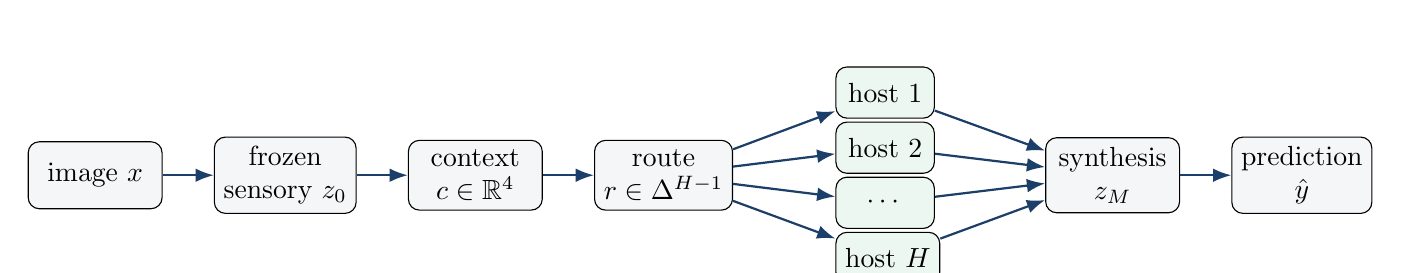
\begin{tikzpicture}[
node distance=0.75cm and 0.65cm,
blk/.style={draw,rounded corners,minimum width=1.7cm,minimum height=0.85cm,align=center,fill=softgray},
host/.style={draw,rounded corners,minimum width=1.25cm,minimum height=0.65cm,align=center,fill=softgreen},
arr/.style={-Latex,thick,deepblue}
]
\node[blk] (x) {image $x$};
\node[blk,right=of x] (z) {frozen\\sensory $z_0$};
\node[blk,right=of z] (c) {context\\$c\in\R^4$};
\node[blk,right=of c] (r) {route\\$r\in\Delta^{H-1}$};
\node[host,right=1.3cm of r,yshift=1.05cm] (h1) {host 1};
\node[host,right=1.3cm of r,yshift=0.35cm] (h2) {host 2};
\node[host,right=1.3cm of r,yshift=-0.35cm] (h3) {$\cdots$};
\node[host,right=1.3cm of r,yshift=-1.05cm] (hh) {host $H$};
\node[blk,right=1.4cm of h2,yshift=-0.35cm] (zm) {synthesis\\$z_M$};
\node[blk,right=of zm] (y) {prediction\\$\hat y$};
\draw[arr] (x)--(z); \draw[arr] (z)--(c); \draw[arr] (c)--(r);
\draw[arr] (r)--(h1); \draw[arr] (r)--(h2); \draw[arr] (r)--(h3); \draw[arr] (r)--(hh);
\draw[arr] (h1)--(zm); \draw[arr] (h2)--(zm); \draw[arr] (h3)--(zm); \draw[arr] (hh)--(zm);
\draw[arr] (zm)--(y);
\end{tikzpicture}%
}
\caption{The internal chain studied by Geometry-MMALS G1. v1.0.9 establishes a candidate geometric result at the context node, but not yet a replicated geometric effect at the route or synthesis nodes.}
\label{fig:pipeline}
\end{figure}

\subsection{Context distance and factor target}

For the same source identity $s$ observed at factors $u_a$ and $u_b$, the normalized half-chord distance is
\begin{equation}
 d_C(c_{s,a},c_{s,b})=\frac12\norm{c_{s,a}-c_{s,b}}_2.
\end{equation}
The factor target over the $120^\circ$ training span is
\begin{equation}
 \tau(u_a,u_b)=
 \sin\left[
 \frac{\pi}{2}
 \min\left(\frac{|u_a-u_b|}{120^\circ},1\right)
 \right].
\end{equation}
This target is compatible with a unit-sphere representation and is independent of curriculum stage.

A local matching loss is
\begin{equation}
 \loss_{C,\mathrm{match}}
 =\E_{s,a,b}
 \left[d_C(c_{s,a},c_{s,b})-\tau(u_a,u_b)\right]^2.
\end{equation}
Far-pair and path-spread terms prevent compressed or nearly constant trajectories:
\begin{align}
 \loss_{C,\mathrm{far}}
 &=\E_{|u_a-u_b|\geq\delta}
 \relu\left(m_C-d_C(c_{s,a},c_{s,b})\right)^2,\\
 \loss_{C,\mathrm{spread}}
 &=\E_s\relu\left(v_{\min}-\frac1{|U|}\sum_{u\in U}
 \norm{c_{s,u}-\bar c_s}_2^2\right)^2.
\end{align}

\subsection{Cross-source fiber alignment}

For adjacent factors, define the source-specific transition
\begin{equation}
 \Delta c_{s,j}=c_{s,u_{j+1}}-c_{s,u_j}.
\end{equation}
The transition must align across source identities for the same interval, not across all intervals with one global direction. A direction-and-length loss is
\begin{equation}
 \loss_{\mathrm{fiber}}=
 \E_j\E_{s\neq s'}
 \left[
 1-\frac{\langle\Delta c_{s,j},\Delta c_{s',j}\rangle}
 {\norm{\Delta c_{s,j}}_2\norm{\Delta c_{s',j}}_2+\varepsilon}
 +\lambda_{\ell}
 \left(\norm{\Delta c_{s,j}}_2-\norm{\Delta c_{s',j}}_2\right)^2
 \right].
\end{equation}
Angle-centroid grounding uses
\begin{equation}
 \bar c_u=\E_s[c_{s,u}],
\end{equation}
and applies the same chord-compatible target to $d_C(\bar c_{u_a},\bar c_{u_b})$. These constraints aim to transform source-specific ordered paths into a more coherent family of fibers.

\subsection{Route geometry}

For route distributions $r_a$ and $r_b$, define square-root simplex coordinates $q=\sqrt r$. The normalized chord distance is
\begin{equation}
 d_R(r_a,r_b)=\frac{\norm{\sqrt{r_a}-\sqrt{r_b}}_2}{\sqrt2}
 =\sqrt{1-\langle\sqrt{r_a},\sqrt{r_b}\rangle}.
\end{equation}
The root-space norm is used numerically because it avoids the singular gradient of $\sqrt{1-\mathrm{affinity}}$ when two routes coincide.

The legacy v1.0.8 route target normalized factor gaps by the maximum gap currently visible in the curriculum. The same angular pair could therefore receive different targets at different continual stages. The stationary v1.0.9 target instead uses $\tau(u_a,u_b)$ above, with a fixed $120^\circ$ span. Its matching and far-separation terms are
\begin{align}
 \loss_{R,\mathrm{match}}
 &=\E_{s,a,b}\left[d_R(r_{s,a},r_{s,b})-\tau(u_a,u_b)\right]^2,\\
 \loss_{R,\mathrm{far}}
 &=\E_{|u_a-u_b|\geq\delta}
 \relu\left(m_R-d_R(r_{s,a},r_{s,b})\right)^2.
\end{align}

\subsection{Complete v1.0.9 training objective}

For aligned treatments, the training objective is
\begin{equation}
\begin{split}
 \loss ={}& \loss_{\mathrm{CE}}
 +\lambda_A\loss_{\mathrm{anchor}}
 +\lambda_R(\loss_{R,\mathrm{match}}+\alpha_R\loss_{R,\mathrm{far}})\\
 &+\lambda_C(\loss_{C,\mathrm{match}}+\alpha_C\loss_{C,\mathrm{far}})
 +\lambda_V\loss_{C,\mathrm{spread}}
 +\lambda_F\loss_{\mathrm{fiber}}
 +\lambda_G\loss_{\mathrm{centroid}}
 +\lambda_H\loss_{\mathrm{host-div}}.
\end{split}
\end{equation}
The no-geometry control retains classification, retention, and host-balance terms but removes the direct geometry terms.

\section{v1.0.9 five-seed experimental protocol}

\subsection{Controlled benchmark}

The factor is image rotation. The training curriculum is
\begin{equation}
 [-60^\circ,-30^\circ,0^\circ,60^\circ,30^\circ].
\end{equation}
The deliberately non-monotonic last two stages test continual adaptation rather than simple traversal. Dense evaluation covers
\begin{equation}
 -75^\circ,-60^\circ,-45^\circ,\ldots,60^\circ,75^\circ.
\end{equation}
Source identities are partitioned so that factor decoding and causal tangent evaluation can be performed on identities excluded from fitting.

\subsection{Matched methods}

Three methods are compared for model seeds $0,1,2,3,4$:
\begin{enumerate}
\item \texttt{d4\_no\_geo}: no direct geometric supervision;
\item \texttt{d4\_full\_legacy\_route}: full d4 alignment with the legacy nonstationary route target;
\item \texttt{d4\_full\_stationary\_route}: full d4 alignment with the fixed stationary route target.
\end{enumerate}
For every seed and method, the run uses $15{,}360$ forward images and $80$ optimizer steps. The sensory split, sensory encoder, source partitions, curriculum, context dimension, host architecture, and initial states are controlled and hashed.

\subsection{Statistics and gates}

Within each seed, paired source-bootstrap intervals estimate effects on geometry, prediction, and causal probes. Across seeds, Student-$t$ intervals treat the model seed as the replication unit. Candidate gates require a positive seed-level confidence bound and a sufficiently high positive-seed fraction. The protocol explicitly separates candidate evidence from final qualification.

\section{Results of v1.0.9}

\subsection{Replicated context geometry}

\begin{figure}[H]
\centering
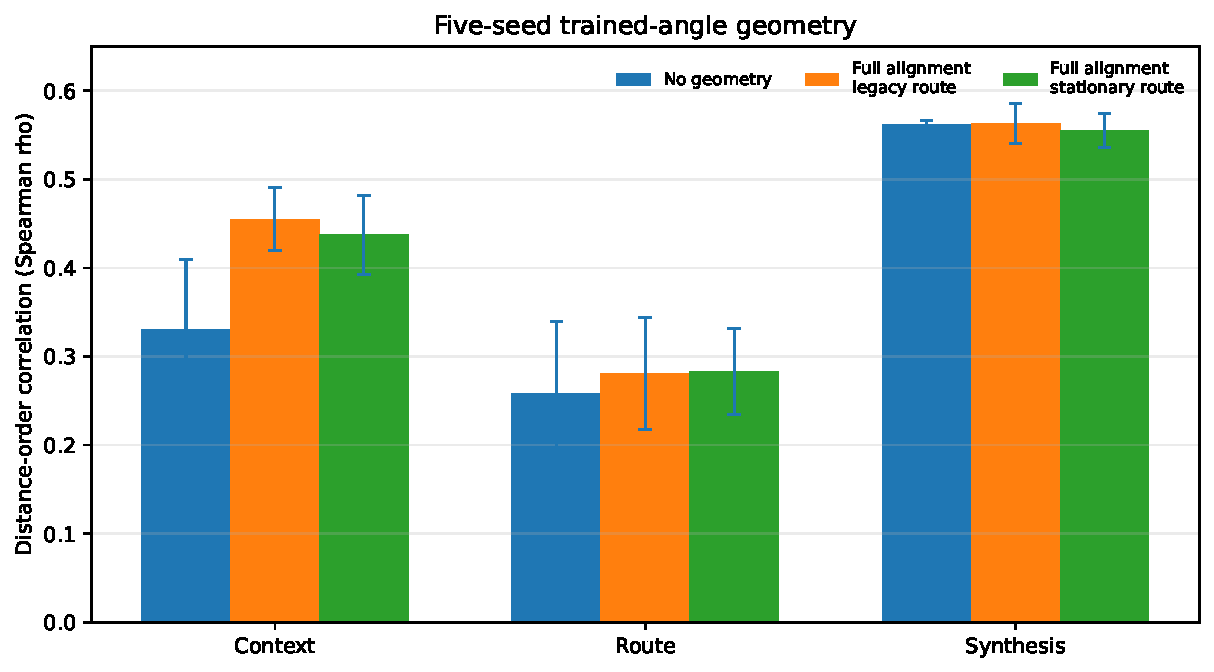
\includegraphics[width=0.86\textwidth]{figures/geometry_summary_v109.pdf}
\caption{Aggregate geometry metrics across five model seeds. The aligned methods improve context order, whereas route and synthesis improvements are not replicated.}
\label{fig:geometry-summary}
\end{figure}

For stationary full alignment versus no geometry,
\begin{equation}
 \Delta\rho_{\mathrm{context}}=+0.107,
 \qquad 95\%\ \mathrm{CI}=[+0.029,+0.185].
\end{equation}
Every seed exhibits a positive context-order effect. Context stress changes by
\begin{equation}
 \Delta\mathrm{stress}_{\mathrm{context}}=-0.042,
 \qquad 95\%\ \mathrm{CI}=[-0.084,-0.001].
\end{equation}
This is the first replicated candidate C1 result of the G1 program.

\begin{figure}[H]
\centering
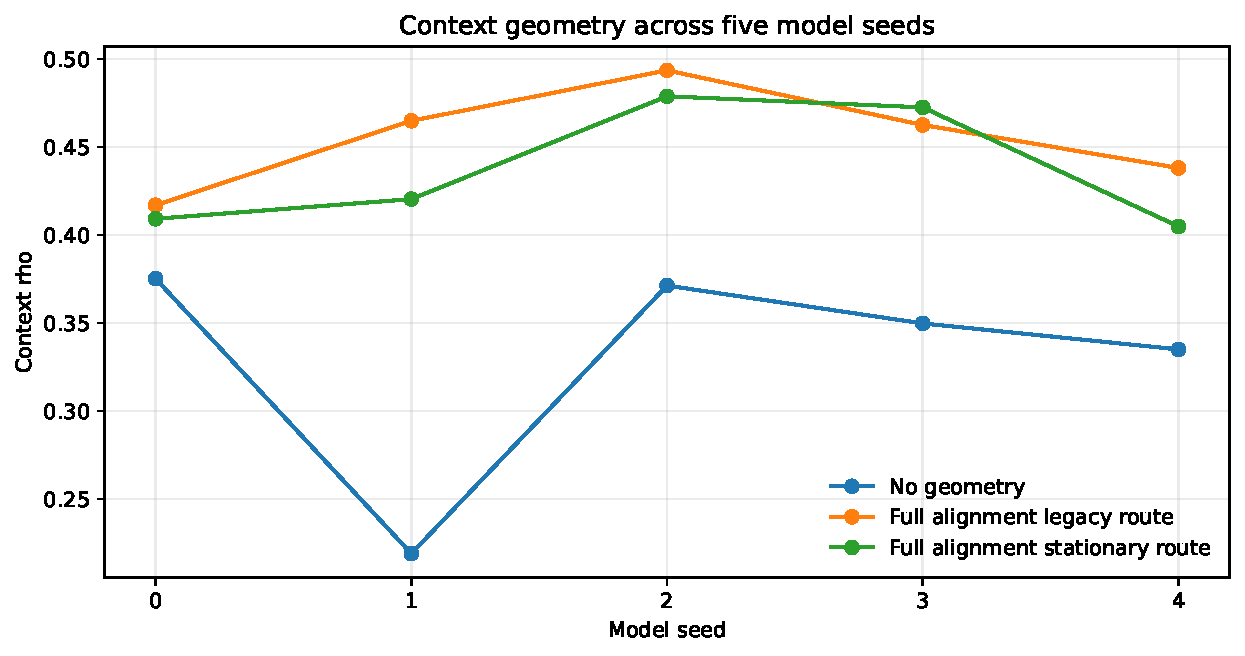
\includegraphics[width=0.88\textwidth]{figures/per_seed_context_v109.pdf}
\caption{Per-seed context distance-order correlation. All five stationary-alignment effects relative to the no-geometry control are positive.}
\label{fig:per-seed-context}
\end{figure}

\subsection{Held-out source decoding improves}

\begin{figure}[H]
\centering
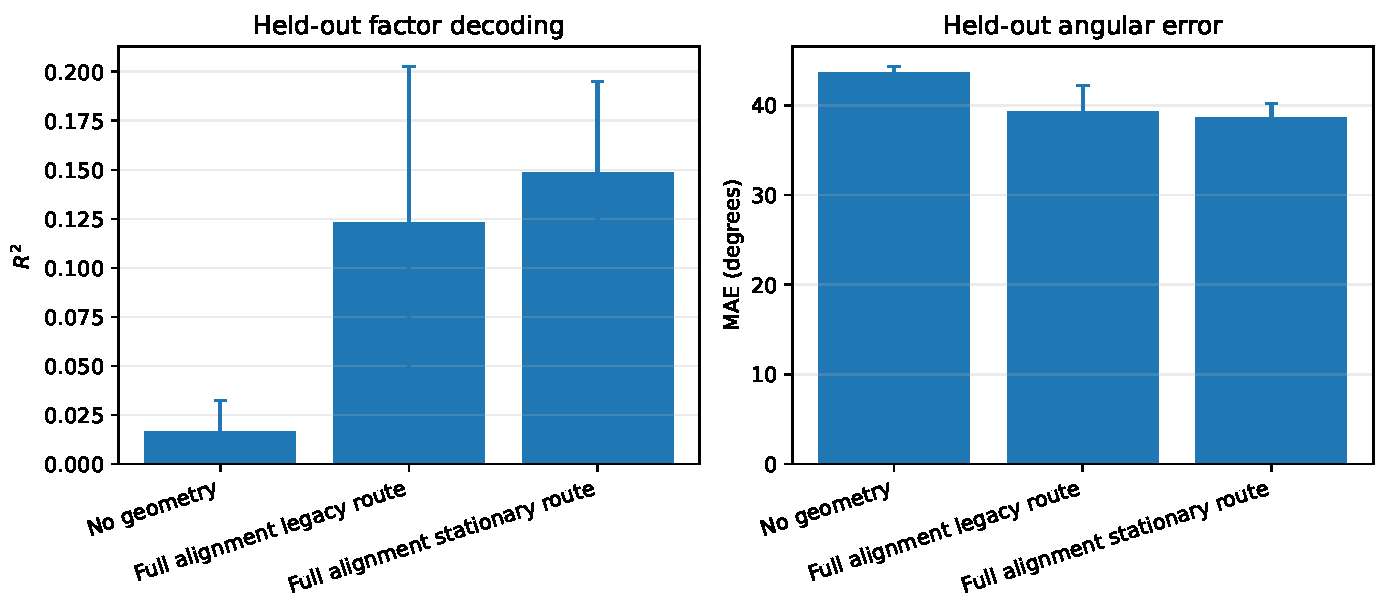
\includegraphics[width=0.86\textwidth]{figures/heldout_decoding_v109.pdf}
\caption{Held-out source factor decoding. The context learned by aligned methods contains more transferable rotation information than the no-geometry control.}
\label{fig:decoding}
\end{figure}

The stationary model reaches mean held-out context $R^2=0.149$, compared with $0.016$ for the no-geometry control. The paired effect is approximately
\begin{equation}
 \Delta R^2=+0.132,
 \qquad 95\%\ \mathrm{CI}=[+0.093,+0.172].
\end{equation}
The mean absolute angle error improves from $43.67^\circ$ to $38.68^\circ$, a reduction of about $4.99^\circ$. Because source identities are disjoint between fitting and evaluation, this is stronger evidence than a training-set embedding visualization.

\subsection{Illustrative context fibers}

\begin{figure}[H]
\centering
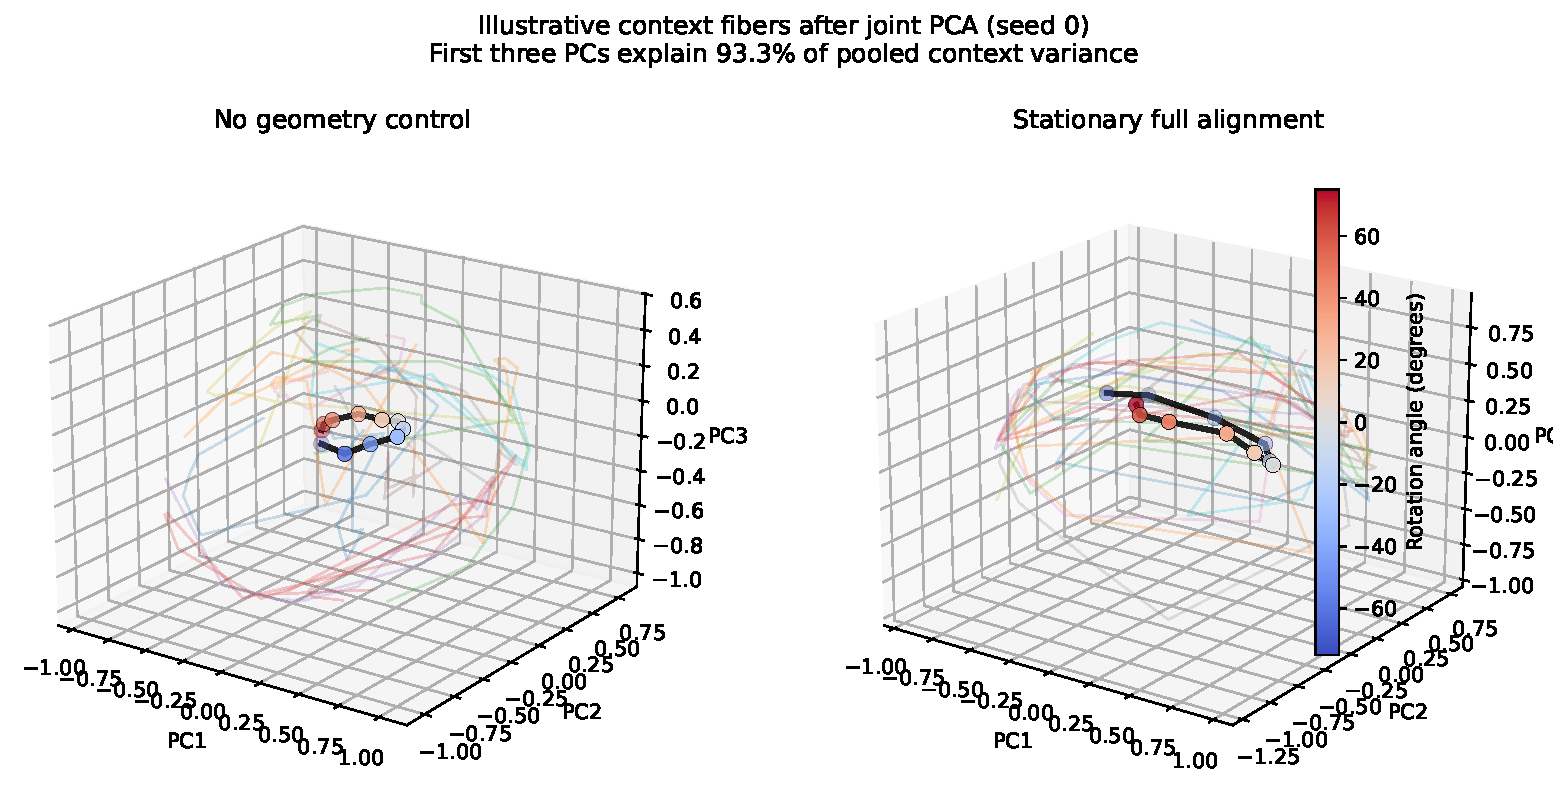
\includegraphics[width=0.98\textwidth]{figures/context_fibers_pca_seed0.pdf}
\caption{Illustrative joint PCA of seed-0 context fibers. Thin curves show selected source identities across dense angles; black curves connect angle centroids. The plot is explanatory rather than a qualification metric because PCA distorts distances. The first three components explain approximately 93.3\% of pooled context variance.}
\label{fig:pca-fibers}
\end{figure}

The expected structure on the current interval is an arc or a family of approximately one-dimensional fibers embedded in $\R^4$, not a torus. A circular topology would require a full periodic factor such as $0^\circ$--$360^\circ$ with closure tests. A torus would require at least two independent periodic factors.

\subsection{The stationary target is cleaner but not empirically superior}

The stationary-versus-legacy contrast is neutral on the main route metric:
\begin{equation}
 \Delta\rho_{\mathrm{route}}=+0.003,
 \qquad 95\%\ \mathrm{CI}=[-0.034,+0.039].
\end{equation}
It is also neutral on context geometry and prediction. The stationary target is theoretically consistent and numerically stable, but this pilot falsifies the claim that it is empirically superior under the tested setting.

\subsection{Route and synthesis geometry do not replicate}

For stationary full alignment versus no geometry,
\begin{align}
 \Delta\rho_{\mathrm{route}}&=+0.025,
 &95\%\ \mathrm{CI}&=[-0.092,+0.142],\\
 \Delta\rho_{\mathrm{synthesis}}&=-0.006,
 &95\%\ \mathrm{CI}&=[-0.025,+0.012].
\end{align}
Only two of five seeds show a positive trained-route effect. Dense held-out route order is also neutral. The replicated chain currently stops at the context representation.

\subsection{Prediction and forgetting remain neutral}

\begin{figure}[H]
\centering
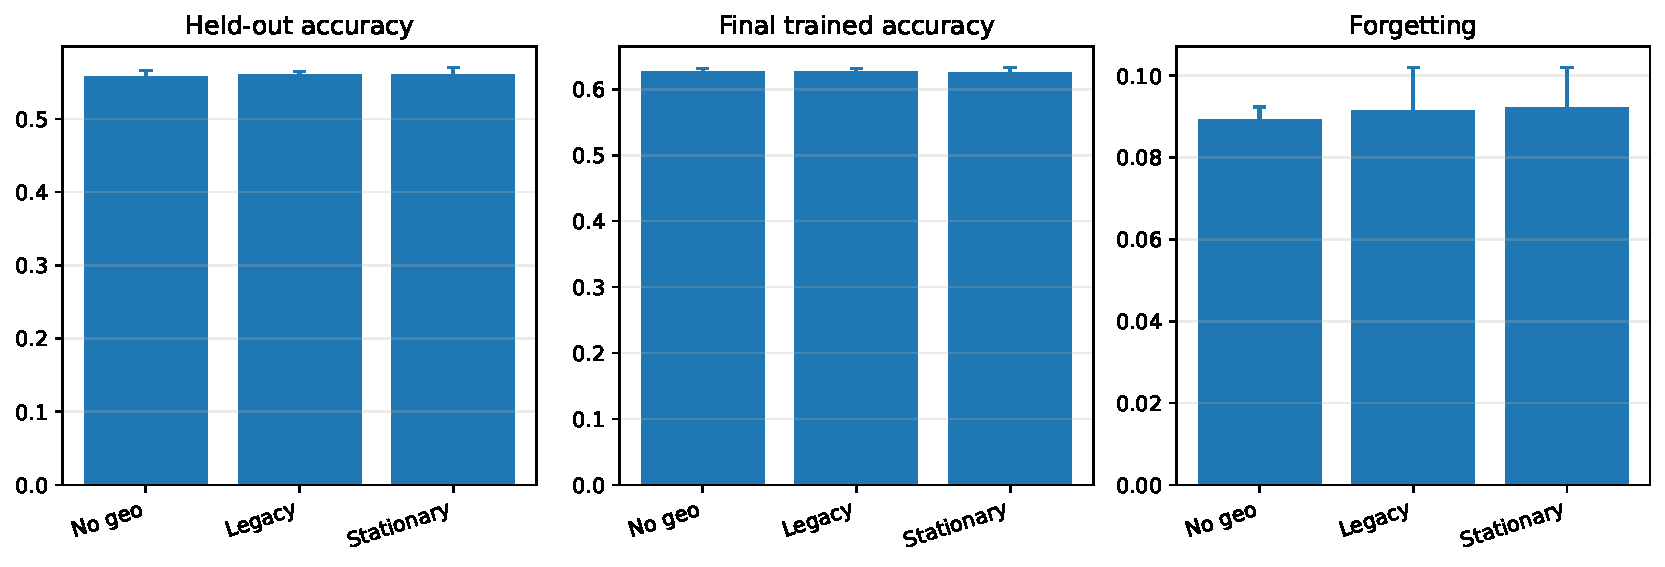
\includegraphics[width=0.86\textwidth]{figures/operational_metrics_v109.pdf}
\caption{Operational metrics across five seeds. Differences in held-out accuracy, final trained accuracy, and forgetting are small and statistically neutral.}
\label{fig:operational}
\end{figure}

The stationary treatment changes mean held-out accuracy by roughly $+0.23$ percentage points, final trained accuracy by $-0.05$ points, and forgetting by $+0.28$ points relative to the no-geometry control. None of the intervals excludes zero. Better measured context geometry therefore does not imply better task performance.

\subsection{Causal specificity does not replicate}

\begin{figure}[H]
\centering
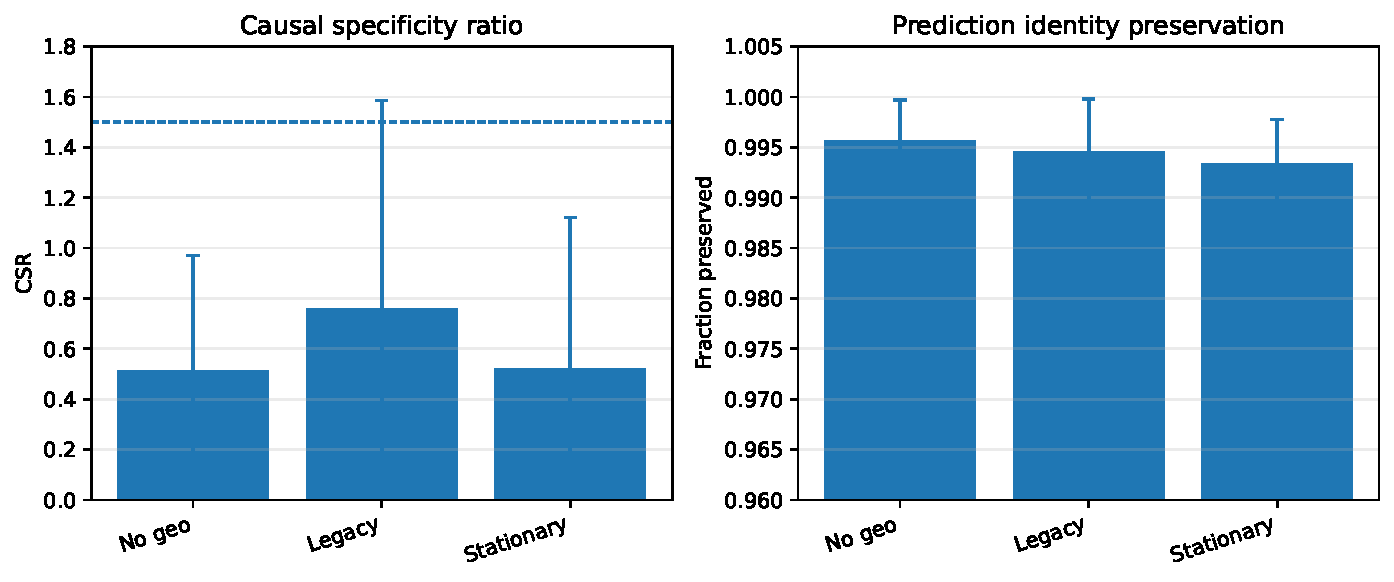
\includegraphics[width=0.86\textwidth]{figures/causal_summary_v109.pdf}
\caption{Aggregate causal probe. Prediction identity is preserved, but tangent interventions are not reliably more route-specific than matched orthogonal interventions.}
\label{fig:causal}
\end{figure}

The stationary model has mean causal-specificity ratio
\begin{equation}
 \mathrm{CSR}=0.523,
 \qquad 95\%\ \mathrm{CI}=[-0.075,1.121],
\end{equation}
well below the candidate threshold $1.5$. Prediction identity is preserved in approximately $99.3\%$ of interventions, but the route response is not directionally specific enough to qualify functional mediation.

\subsection{Current gate table}

\begin{table}[H]
\centering
\caption{v1.0.9 gate status.}
\begin{tabularx}{\textwidth}{@{}Y C Y@{}}
\toprule
Gate & Result & Interpretation\\
\midrule
C0 equal compute across all seeds & Pass & Protocol integrity\\
C1 stationary context geometry & Candidate pass & Seed CI excludes zero\\
C1 stationary route geometry & Fail & Route effect not replicated\\
Stationary target beats legacy & Fail & Theoretical correction, no empirical superiority\\
C2 predictive superiority & Fail & Accuracy and forgetting neutral\\
C3 host specialization & Not evaluated & No replicated ecology test\\
C4 causal specificity & Fail & CSR below threshold\\
C4 prediction identity preservation & Candidate pass & Interventions mostly preserve class\\
C5 memory transport & Not implemented & Future work\\
C6 operational utility & Not qualified & No measured advantage\\
\bottomrule
\end{tabularx}
\end{table}

\section{Interpretation: what has and has not been learned}

\subsection{A real advance}

The architecture is capable of learning a low-dimensional internal context whose relations correspond to rotation and generalize across source identities. That eliminates one major uncertainty. The program is not blocked at the representation stage.

\subsection{The functional gap}

The desired chain is
\begin{equation}
 \text{factor}\rightarrow c\rightarrow r\rightarrow\{g_h\}\rightarrow z_M\rightarrow\hat y.
\end{equation}
The evidence supports the first arrow at candidate level, but not the remainder. Three explanations remain open:
\begin{enumerate}
\item the MLP router uses information in $c$ without preserving its metric order;
\item route distributions possess a natural geometry different from the present Hellinger/root-chord metric;
\item hosts are functionally too similar, so large nominal route changes may be irrelevant and small changes toward a distinct host may matter greatly.
\end{enumerate}

This third explanation motivates a functional route metric. If hosts 1 and 2 perform nearly the same transformation, moving probability mass from one to the other should be cheap. A coordinate-wise simplex metric cannot know this.

\subsection{Representational, functional, and operational geometry}

\begin{mathbox}[Three distinct scientific claims]
\begin{align*}
\text{Representational: }& d_C(c_a,c_b)\ \text{reflects factor relations}.\\
\text{Functional: }& \delta c\ \text{causes structured changes in routes and host contributions}.\\
\text{Operational: }& \text{the resulting chain improves a task, retention, robustness, or cost}. 
\end{align*}
\end{mathbox}

The v1.0.9 result is valuable precisely because it separates these claims rather than allowing an attractive latent plot to stand in for all three.

\section{Complete Geometry-MMALS G1 v1.1.0 specification}

\subsection{Research question}

\begin{plainbox}[Primary v1.1.0 question]
Can an explicitly geometry-mediated router convert the replicated context representation into ordered, causally specific, and functionally meaningful changes in host allocation?
\end{plainbox}

The target chain is
\begin{equation}
 u\longrightarrow c\longrightarrow r\longrightarrow g_h\longrightarrow z_M.
\end{equation}
Version 1.1.0 is a bridge experiment, not a full ecosystem release. It does not yet introduce heterogeneous host architectures, bottom-up host state, dynamic loss regulation, reinforcement learning, or memory transport.

\subsection{Core design principle: freeze the success already obtained}

For each model seed, v1.1.0 begins from a v1.0.9-aligned d4 context checkpoint. The frozen modules are
\begin{equation}
 P\ \text{and}\ C_\phi.
\end{equation}
Thus $z_0$ and $c$ are identical across router treatments for the same input. Router, hosts, and classifier are initialized from matched states and trained under equal compute. This separates the question ``can the context geometry be learned?'' from ``can a router use it?''

The primary routing phase must not use the true angle label. Angle labels are permitted only for evaluation metrics and for fitting causal tangent probes on designated source partitions.

\subsection{Primary router family}

Three routers are compared.

\subsubsection{R0: current MLP context router}

\begin{equation}
 \ell^{(0)}(c)=W_2\phi(W_1c+b_1)+b_2,
 \qquad r^{(0)}(c)=\softmax\left(\ell^{(0)}(c)/\tau\right).
\end{equation}
This is the current flexible baseline. It can use context information without preserving context geometry.

\subsubsection{R1: low-capacity linear router}

\begin{equation}
 \ell^{(1)}(c)=Wc+b,
 \qquad r^{(1)}(c)=\softmax\left(\ell^{(1)}(c)/\tau\right).
\end{equation}
The linear router tests whether a simple transformation can transmit the learned context order. Its lower capacity is intentional and must be reported. A supplementary parameter-matched MLP sanity check is permitted but is not a primary treatment.

\subsubsection{R2: prototype-energy router}

Each host has a normalized context prototype $\mu_h\in S^{d_c-1}$ and positive bandwidth $\sigma_h$:
\begin{equation}
 \norm{\mu_h}_2=1,
 \qquad \sigma_h=\sigma_{\min}+\operatorname{softplus}(s_h).
\end{equation}
The geometric energy is
\begin{equation}
 E_h^{\mathrm{geo}}(c)=
 \frac{d_C(c,\mu_h)^2}{2\sigma_h^2}+b_h.
\end{equation}
The route is
\begin{equation}
 r_h^{(2)}(c)=
 \frac{\exp[-E_h^{\mathrm{geo}}(c)/\tau]}
 {\sum_k\exp[-E_k^{\mathrm{geo}}(c)/\tau]}.
\end{equation}
Prototypes are initialized by spherical $k$-means on training contexts without angle labels. Bandwidths are initialized from within-cluster distances. Prototypes and bandwidths remain trainable, with projection of $\mu_h$ back to the unit sphere after each optimizer step.

\begin{positivebox}[Connection to the previously planned energy-guided router]
The prototype router is not a competing direction. It is the first controlled implementation of the geometric term in the broader energy-guided router:
\begin{equation}
 E_h=\alpha E_h^{\mathrm{geo}}+\beta E_h^{\mathrm{host}}+
 \gamma E_h^{\mathrm{memory}}+\delta E_h^{\mathrm{cost}}+
 \eta E_h^{\mathrm{goal}}.
\end{equation}
Version 1.1.0 implements only $E_h^{\mathrm{geo}}$. Later G2 stages add host state, memory risk, cost, stability, and goal conditioning. Reinforcement learning and forward--backward control operate at a still later temporal-control level.
\end{positivebox}

\subsection{Common training objective}

Because the context encoder is frozen, the primary routing experiment uses
\begin{equation}
 \loss_{\mathrm{route-phase}}=
 \loss_{\mathrm{CE}}
 +\lambda_A\loss_{\mathrm{anchor}}
 +\lambda_B\loss_{\mathrm{balance}}
 +\lambda_D\loss_{\mathrm{host-div}}.
\end{equation}
The same loss and coefficients are used for R0, R1, and R2. No angle-supervised route-geometry loss is applied in the primary comparison. This is essential: R2 must demonstrate mediation because its architecture uses context distance, not because the answer is directly imposed on its route outputs.

Usage balancing may be written
\begin{equation}
 \loss_{\mathrm{balance}}=
 \sum_{h=1}^{H}
 \left(\E_x[r_h(x)]-\frac1H\right)^2.
\end{equation}
Host diversity remains weak and identical across treatments. It is not used to force a predetermined specialization pattern.

\subsection{Nominal route geometry}

For historical comparability, route differences are measured with the root-simplex chord
\begin{equation}
 d_R(r_a,r_b)=\frac{\norm{\sqrt{r_a}-\sqrt{r_b}}_2}{\sqrt2}.
\end{equation}
Metrics include source-level Spearman correlation with factor gaps, stress, dense held-out interpolation order, route entropy, and transition smoothness.

\subsection{Functional route geometry}

Nominal coordinates treat host indices as equally distinct. v1.1.0 therefore estimates a host-function cost matrix. Let
\begin{equation}
 v_h(x)=g_h(z_0(x)).
\end{equation}
The primary cost is
\begin{equation}
 C_{hk}=\E_{x\in\mathcal{D}_{\mathrm{metric}}}
 \left[
 \frac{\norm{v_h(x)-v_k(x)}_2^2}{d_M}
 \right],
\end{equation}
where $\mathcal{D}_{\mathrm{metric}}$ is a fixed held-out metric set and $d_M$ is the synthesis dimension. The matrix is symmetrized and scaled by its nonzero median.

The functional distance between two routes is the entropically regularized optimal-transport cost
\begin{equation}
 W_C^\varepsilon(r_a,r_b)=
 \min_{\Pi\geq0}
 \left\langle \Pi,C\right\rangle
 +\varepsilon\KL\!\left(\Pi\middle\|r_ar_b^\top\right)
\end{equation}
subject to
\begin{equation}
 \Pi\mathbf{1}=r_a,
 \qquad
 \Pi^\top\mathbf{1}=r_b.
\end{equation}
This Sinkhorn-computable metric asks how costly it is to transform one host coalition into another given what the hosts actually do. It is an evaluation metric in v1.1.0, not a training loss, avoiding circular optimization.

A supplementary ablation-derived cost may be reported:
\begin{equation}
 C^{\mathrm{abl}}_{hk}=\E_x
 \left|\Delta\ell_h(x)-\Delta\ell_k(x)\right|,
\end{equation}
where $\Delta\ell_h$ is the true-class log-probability change after ablating host $h$.

\subsection{Low-capacity mediation probes}

A simple probe tests whether route variation is explainable from context structure. Because $\sqrt r$ lies on the positive unit sphere, fit
\begin{equation}
 \widehat q=A c+b,
 \qquad
 \widehat r=\frac{[\widehat q]_+^2}{\sum_h[\widehat q_h]_+^2+\varepsilon}.
\end{equation}
The probe is trained on designated source identities and trained angles, then evaluated on held-out identities and dense unseen angles. Report:
\begin{itemize}
\item $R^2$ for predicting $\sqrt r$;
\item root-chord route error;
\item functional transport error $W_C^\varepsilon(\widehat r,r)$;
\item performance after angle-label shuffling;
\item performance after replacing the context tangent component with an orthogonal component.
\end{itemize}
A high in-sample score alone is not evidence. Generalization and controls are mandatory.

\subsection{Differential and causal mediation}

Let $t(c)$ be a local unit tangent corresponding to increasing rotation, estimated from context centroids on a fit partition. Let $v_j(c)$ be matched unit directions orthogonal to $t(c)$. The router Jacobian in root-simplex coordinates is
\begin{equation}
 J_q(c)=\frac{\partial\sqrt{r(c)}}{\partial c}.
\end{equation}
Define tangent and orthogonal sensitivities
\begin{align}
 S_t(c)&=\norm{J_q(c)t(c)}_2,\\
 S_\perp(c)&=\frac1J\sum_{j=1}^{J}\norm{J_q(c)v_j(c)}_2.
\end{align}
The differential mediation ratio is
\begin{equation}
 \mathrm{DMR}=\frac{\E[S_t]}{\E[S_\perp]+\varepsilon}.
\end{equation}

Finite interventions use
\begin{equation}
 c_t^\pm=\operatorname{normalize}(c\pm\epsilon t),
 \qquad
 c_{\perp,j}^+=\operatorname{normalize}(c+\epsilon v_j).
\end{equation}
Report nominal and functional causal-specificity ratios:
\begin{align}
 \mathrm{CSR}_{\mathrm{nom}}
 &=\frac{\E[d_R(r(c_t^+),r(c))]}
 {\E_j[d_R(r(c_{\perp,j}^+),r(c))]+\varepsilon},\\
 \mathrm{CSR}_{\mathrm{func}}
 &=\frac{\E[W_C^\varepsilon(r(c_t^+),r(c))]}
 {\E_j[W_C^\varepsilon(r(c_{\perp,j}^+),r(c))]+\varepsilon}.
\end{align}
Signed consistency compares $c_t^+$ and $c_t^-$ and requires reproducible opposite displacement along a learned route coordinate. Prediction identity and true-class log probability are monitored to distinguish a controlled route change from destructive perturbation.

\subsection{Host ecology measurements}

Version 1.1.0 measures specialization rather than forcing it. For factor $u$, define host territory
\begin{equation}
 A_h(u)=\E_s[r_h(c_{s,u})].
\end{equation}
Normalize across factors:
\begin{equation}
 p_h(u)=\frac{A_h(u)}{\sum_{u'}A_h(u')+\varepsilon}.
\end{equation}
An entropy-based specialization score is
\begin{equation}
 \mathrm{Spec}_h=1-\frac{H(p_h)}{\log|U|},
 \qquad H(p_h)=-\sum_u p_h(u)\log p_h(u).
\end{equation}
It is zero for uniform use and approaches one for a narrow territory.

Territory overlap is
\begin{equation}
 O_{hk}=\sum_u\min(p_h(u),p_k(u)).
\end{equation}
Functional diversity uses $C_{hk}$, while redundancy is the combination of high overlap and low functional cost. Host ablation at factor $u$ is
\begin{equation}
 \Delta\mathrm{Acc}_h(u)=
 \mathrm{Acc}(u)-\mathrm{Acc}_{-h}(u).
\end{equation}
A genuine host ecology should show structured territories and factor-dependent ablation effects rather than mere differences in route mass.

\subsection{Experimental matrix}

The primary pilot uses five paired model seeds. For each seed:
\begin{enumerate}
\item load or reproduce the same aligned d4 context checkpoint;
\item freeze $P$ and $C_\phi$;
\item create matched initial states for hosts and classifier;
\item train R0, R1, and R2 under identical curriculum, batches, forward budget, optimizer steps, anchor schedule, and early-stopping policy;
\item evaluate on trained angles, dense unseen angles, held-out source identities, and source-disjoint intervention partitions.
\end{enumerate}

The primary contrasts are
\begin{align}
 \mathrm{R2}-\mathrm{R0}&:\ \text{structural geometric routing versus flexible MLP},\\
 \mathrm{R2}-\mathrm{R1}&:\ \text{prototype energy versus low-capacity linear mediation},\\
 \mathrm{R1}-\mathrm{R0}&:\ \text{effect of capacity and linearity}.
\end{align}
A ten-seed qualification run is permitted only if the five-seed pilot passes the functional mediation gates.

\subsection{Statistical plan}

Within a seed, source identities are the bootstrap unit. Across seeds, report paired mean effects, Student-$t$ 95\% intervals, standard deviation, and positive-seed fraction. Multiple primary route metrics must be declared before execution. Angle-wise prediction effects are secondary and should use false-discovery-rate control.

No source identity used to fit the context tangent, probe, prototype initialization diagnostics, or host cost matrix may be reused as the final causal evaluation unit.

\subsection{Candidate gates and falsification conditions}

\begin{table}[H]
\centering
\caption{Preregistered candidate gates for v1.1.0.}
\begin{tabularx}{\textwidth}{@{}Y Y@{}}
\toprule
Gate & Candidate requirement\\
\midrule
Context preservation & Frozen-context geometry and held-out decoding remain within numerical tolerance of the source checkpoint\\
Nominal route mediation & R2--R0 route-order effect has seed CI lower bound $>0$ and at least $4/5$ positive seeds\\
Functional route mediation & R2--R0 functional-route order or tangent transport effect has seed CI lower bound $>0$\\
Causal specificity & Source-bootstrap lower bound of $\mathrm{CSR}_{\mathrm{func}}>1$ and seed mean target $>1.5$\\
Low-capacity generalization & Held-out route-probe error improves over shuffled and orthogonal controls\\
Host ecology & R2 increases specialization or factor-dependent ablation structure without total host collapse\\
Safety / preservation & Prediction identity lower bound $\geq0.95$ under causal probes\\
Operational non-degradation & Final accuracy and forgetting are not worse than R0 by more than a preregistered equivalence margin of one percentage point\\
\bottomrule
\end{tabularx}
\end{table}

The primary hypothesis is falsified if R2 does not improve either nominal or functional route mediation over R0 across seeds. If nominal geometry remains neutral but functional transport improves, the previous route metric was incomplete. If both remain neutral, the prototype architecture does not build the bridge. If route mediation improves but host ablation and synthesis remain neutral, the bridge reaches routing but not function.

\subsection{Preregistered secondary intervention}

The main experiment does not train with a mediation loss. If R2 fails the primary mediation gate, a separately reported secondary arm may test
\begin{equation}
 \loss_{\mathrm{med}}=
 \relu\left(m_{\mathrm{med}}-
 d_{\mathrm{func}}(r(c+\epsilon t),r(c))+
 d_{\mathrm{func}}(r(c+\epsilon v_\perp),r(c))
 \right),
\end{equation}
where $d_{\mathrm{func}}=W_C^\varepsilon$. This arm must not be pooled with the architecture-only result. It answers a different question: whether mediation can be directly trained rather than structurally induced.

\subsection{Artifact and reproducibility contract}

The v1.1.0 notebook must export, for every seed and router:
\begin{itemize}
\item frozen-context checkpoint hashes and matched initial-state hashes;
\item compute and wall-time summaries;
\item nominal and functional route-geometry tables;
\item host cost matrices and their construction partitions;
\item low-capacity probe metrics and controls;
\item Jacobian sensitivity and finite-intervention results;
\item host territory, overlap, specialization, functional diversity, and ablation tables;
\item prediction, NLL, forgetting, and retention tables;
\item source-bootstrap and seed-level aggregate effects;
\item a machine-readable gate summary and claim manifest.
\end{itemize}
The package must archive all analysis code, fixed configuration, environment capture, results, figures, and a no-overclaim statement.

\section{What remains after v1.1.0}

\subsection{G1.2: host ecology}

If v1.1.0 establishes $c\rightarrow r$, the next objective is
\begin{equation}
 c\rightarrow r\rightarrow g_h\rightarrow z_M.
\end{equation}
G1.2 should test heterogeneous or differentiated hosts, overlapping territories, protective redundancy, targeted ablation, and recovery. Functional diversity and redundancy are competing requirements and must be measured separately.

\subsection{G1.3: geometry-aware memory transport}

The next claim concerns preservation or controlled movement of functions through continual updates. Optimal transport can compare host coalitions and context fibers before and after learning. Required evidence includes endpoint checkpoints, repeated post-hoc evaluation, transport cost, retention, and intervention stability.

\subsection{G2: full energy-guided routing}

The prototype term becomes one component of a richer energy:
\begin{equation}
 E_h(c,m,g,s_h)=
 \alpha E_h^{\mathrm{geo}}(c)
 +\beta E_h^{\mathrm{uncertainty}}(s_h)
 +\gamma E_h^{\mathrm{cost}}(s_h)
 +\delta E_h^{\mathrm{memory}}(m)
 +\eta E_h^{\mathrm{stability}}(m,s_h)
 +\zeta E_h^{\mathrm{goal}}(g).
\end{equation}
Here $s_h$ is bottom-up host state, $m$ is memory state, and $g$ is the current objective. The route remains
\begin{equation}
 r_h\propto\exp[-E_h/\tau].
\end{equation}
This is compatible with dynamic goals such as accuracy, retention, cost, drift stability, or specialization.

\subsection{G2.1: bottom-up host feedback and distributed control}

Hosts should eventually report uncertainty, novelty, saturation, available capacity, and error. The router then arbitrates offers and constraints rather than acting as a purely central decision maker. This is the first concrete step toward the mycelial, bidirectional architecture envisioned by MMALS.

\subsection{G2.2: temporal control and reinforcement learning}

A meta-router may optimize future consequences:
\begin{equation}
 Q(s,r)=\E\left[\sum_{t=0}^{T}\gamma^t R_t\right].
\end{equation}
Forward--backward control compares reachable future states with a goal vector. These methods are complementary to geometric routing: geometry structures the action space, while RL or predictive control selects routes under future objectives.

\subsection{G3: phase-aware and quantum-inspired routing}

Only after functional geometry, host ecology, and memory transport are established should the program test amplitudes, phases, interference, or density-matrix representations of route uncertainty. These are quantum-inspired mathematical models, not claims of quantum hardware or quantum advantage.

\section{Limitations}

The benchmark uses a controlled synthetic transformation and a small number of model seeds. Rotation labels shape the context geometry during training, so the result is supervised geometric grounding rather than unsupervised discovery. The context result does not identify a unique global manifold and is invariant to coordinate isometries. PCA visualizations are illustrative. Hosts are currently homogeneous residual modules. The route metric may not reflect host function, which is a central motivation for v1.1.0. Finally, predictive neutrality means that the current geometry is scientifically observable but not yet operationally justified.

\section{Conclusion}

Geometry-MMALS G1 v1.0.9 reaches a genuine but carefully bounded milestone. Across five matched-compute seeds, the system learns a more ordered four-dimensional context representation and transfers rotation information to unseen source identities. This establishes that the architecture can construct a grounded representational geometry. It does not establish that the router, hosts, or synthesis use that geometry in a reproducible functional way.

The next step is therefore not another attempt to raise context correlation in isolation. Version 1.1.0 freezes the successful context representation and tests three router designs, including a prototype-energy router that is the geometric core of the broader energy-guided architecture. It introduces a functional optimal-transport metric over hosts, low-capacity mediation probes, tangent-versus-orthogonal interventions, and host-ecology measurements. The experiment is designed so that every possible outcome is informative: success would establish the first causal bridge toward functional geometry; failure would identify whether the problem lies in the router architecture, the host ecology, or the measurement of route function.

\appendix
\section{Exact v1.0.9 evidence snapshot}

\begin{table}[H]
\centering
\caption{Aggregate v1.0.9 method summary across five seeds.}
\begin{tabular}{@{}lrrr@{}}
\toprule
Metric & No geometry & Legacy full & Stationary full\\
\midrule
Context $\rho$ & 0.330 & 0.455 & 0.437\\
Route $\rho$ & 0.258 & 0.280 & 0.283\\
Synthesis $\rho$ & 0.562 & 0.563 & 0.555\\
Dense context $\rho$ & 0.283 & 0.348 & 0.332\\
Dense route $\rho$ & 0.227 & 0.217 & 0.221\\
Held-out context $R^2$ & 0.016 & 0.123 & 0.149\\
Held-out angle MAE & $43.67^\circ$ & $39.34^\circ$ & $38.68^\circ$\\
Mean held-out accuracy & 0.558 & 0.561 & 0.561\\
Final trained accuracy & 0.626 & 0.626 & 0.626\\
Mean forgetting & 0.089 & 0.092 & 0.092\\
\bottomrule
\end{tabular}
\end{table}

\section{Notation bridge}

\begin{longtable}{@{}p{0.17\textwidth}p{0.75\textwidth}@{}}
\toprule
Symbol & Meaning\\
\midrule
$x$ & input image\\
$z_0=P(x)$ & frozen sensory representation\\
$c_{\mathrm{raw}}$ & unnormalized inferred context\\
$c$ & normalized functional context\\
$u$ & controlled rotation factor\\
$r$ & route distribution over hosts\\
$g_h$ & host transformation\\
$z_M$ & weighted synthesis of host outputs\\
$\mu_h,\sigma_h$ & prototype center and territory width of host $h$\\
$C_{hk}$ & functional cost between hosts $h$ and $k$\\
$W_C^\varepsilon$ & entropic optimal-transport distance between routes\\
$t(c)$ & local context tangent associated with increasing factor\\
CSR / DMR & finite causal-specificity and differential mediation ratios\\
\bottomrule
\end{longtable}

\section{Repository status language}

The recommended repository status after this release is:

\begin{quote}
Geometry-MMALS G1 v1.0.9 provides replicated candidate evidence for grounded representational context geometry across five matched-compute model seeds. The result generalizes to held-out source identities but does not extend reliably to route geometry, synthesis, prediction, forgetting, or causal specificity. The repository includes a complete v1.1.0 specification for testing geometry-mediated functional routing. v1.1.0 is a protocol specification and has not yet been executed.
\end{quote}

\printbibliography
\end{document}
